\section{Evaluation Concept}
\label{sec:exp_prelim_evaluation_concept}

\begin{figure}[t]
    \centering
    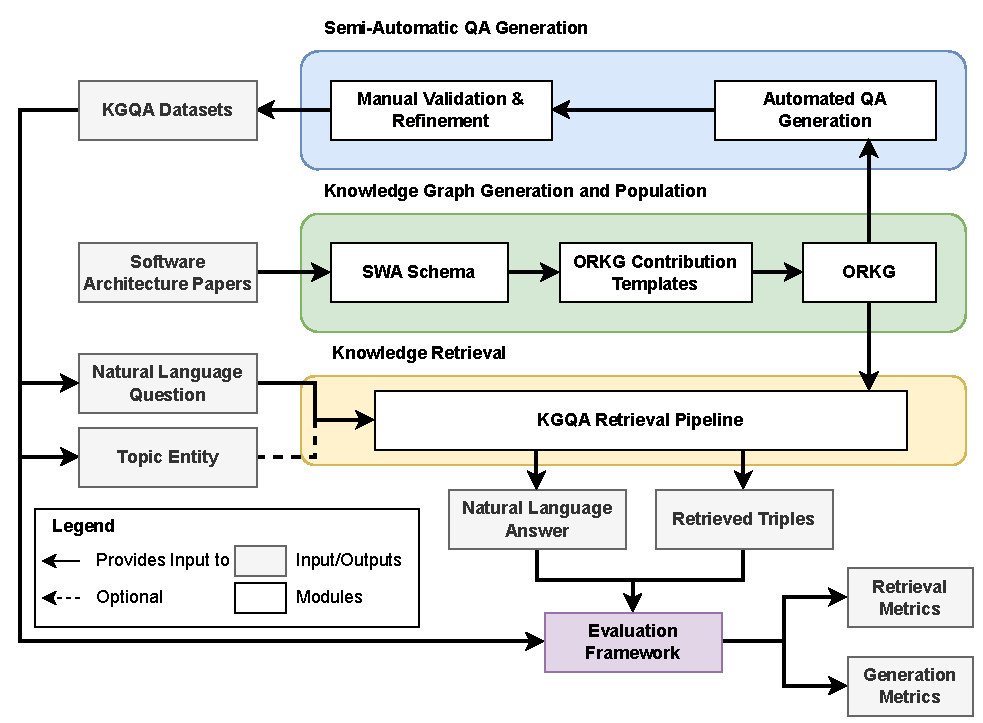
\includegraphics[width=0.95\textwidth]{figures/experiments/orkg/figures-imp_concept_exp.drawio.pdf}
    \caption[Evaluation Concept for Evaluating HubLink on the ORKG]{The overall evaluation concept that we used to perform the experiments on the \gls{orkg} using the proposed HubLink approach and the implemented \gls{kgqa} baseline approaches.}
    \label{fig:implementation_concept}
\end{figure}

This section details the evaluation concept, which we used to perform the evaluation with the objective of assessing the performance of our proposed HubLink approach. The primary objective of this concept is to systematically compare the capabilities of the HubLink retriever against established baseline methods. As indicated in Section~\ref{sec:implementation_orkg}, the \gls{orkg} serves as the underlying \gls{rkg} for these experiments. Furthermore, the \gls{karagen} method \cite{kaplan_combining_2024}, designed for implementing an \gls{llm}-based \gls{qa} system on the \gls{orkg}, forms the basis of the experimental setup. This framework is particularly suitable, as it encompasses the necessary components for applying a \gls{kgqa} retriever to the \gls{orkg}, including data population and retrieval processes. \autoref{fig:implementation_concept} provides a visual overview of the complete experimental design, which we detail in the following.

The general experimental concept starts with the \emph{Knowledge Graph Generation and Population} module. This module is proposed by the \gls{karagen} method and includes the preparation of contribution templates to populate the \gls{orkg} with data. We prepared four such templates, which are described in Section~\ref{sec:contribution_templates}. We fill these templates with data using the \gls{swa} schema detailed in Section~\ref{sec:implementation_orkg}. These populated templates are used by the \gls{sqa} system to automatically fill in the publication data in the \gls{orkg}.

The next module in the evaluation concept is \emph{Knowledge Retrieval}, which also aligns with the principles described in the \gls{karagen} method. In our implementation, the \gls{sqa} system is employed to construct the \gls{kgqa} retrieval pipeline. This enables systematic experimentation by providing a dynamic configuration setup where parameters and pipeline steps can be easily exchanged. The pipeline accepts a natural language question as input and, optionally, a topic entity serving as an entry point into the \gls{orkg}. It then performs knowledge retrieval utilizing either the HubLink retriever or one of five baseline \gls{kgqa} approaches from the literature, detailed in Section~\ref{sec:implementation_baselines}. The parameters that are used for these approaches are chosen by the \emph{Parameter Selection Process}, which is documented in \autoref{ch:parameter_selection_process}. The outputs of the \emph{Knowledge Retrieval} module are a natural language answer and the list of triples retrieved from the graph. These two types of outputs allow the evaluation of both the generation and the retrieval parts of the \gls{kgqa} approach.

The inputs to this system (question and topic entity) are automatically provided to the \gls{kgqa} approach by the \gls{kgqa} dataset. This dataset is the output of the \emph{Semi-Automatic QA Generation} module. Here, the \gls{qa} generation processes implemented in the \gls{sqa} system are used for the generation of \gls{kgqa} pairs (see Section~\ref{sec:implementation_qa_dataset_generation}). During generation, questions are generated in a controlled manner with \gls{llm} assistance using the \gls{orkg} subgraph as the data source. Furthermore, ground-truth data is generated, which is required for the subsequent evaluation phase.

Following the execution of the retrieval pipeline, the output is evaluated within the \emph{Evaluation Framework} module. This final module employs the generated ground-truth data to compute relevant performance metrics. Analysis of these metrics facilitates drawing conclusions regarding the effectiveness and performance characteristics of the evaluated \gls{kgqa} approaches.